\begin{frame}{}
\begin{large}
\begin{center}
B.1 Basics of Structural Approaches: C-CAPM
\end{center}
\end{large}
\end{frame}


\begin{frame}
\begin{footnotesize}
\begin{itemize}
	\item {\color{blue}Structural models} link the stochastic discount factor (s.d.f.) [Slide \ref{slide:AAOSDF}] to investor behaviour through assumptions about preferences.
	\item Investors make portfolio decisions to obtain a desired time and risk profile of consumption.
	\item The s.d.f. $M_{t,t+1}$ captures the aspects of utility that matter for valuing the assets.
	\item Example: C-CAPM [\href{http://www.people.hbs.edu/rmerton/Intertemporal\%20Capital\%20Asset\%20Pricing\%20Model.pdf}{Merton (1973)}, \href{http://www.sciencedirect.com/science/article/pii/0304405X79900163}{Breeden (1979)}]
	
	\item It extends the CAPM framework by providing a consumption-based theory of the determinants of the valuation of the market portfolio.
	
	\item Basic version: representative investor with {\color{blue}time-additive preferences} acting in a complete market.
	
	\item It has been extended in several directions: more complex investor preferences [e.g. Epstein-Zin, Slide \ref{slide:EpsteinZin_def}], investor heterogeneity, incomplete markets, borrowing restrictions.
\end{itemize}
\end{footnotesize}
\end{frame}



\begin{frame}
\begin{footnotesize}
\begin{itemize}
%	\item Dynamic asset pricing models build on optimizing behavior, implying arbitrage-free prices.
%	\item In a dynamic model, risk preferences of investors can vary over time, for instance as a result of consumption or wealth shocks, thus generating fluctuations in risk premia and predictability of returns.
	\item Representative agent maximizes expected utility [Def. \ref{def:EUTSpref}]:
	$$
	U_t = \mathbb{E}_t \left[ \sum_{j=0}^\infty \delta^j u(C_{t+j}) \right],
	$$
	where $u$ is a utility function of consumption and $\delta$ is the subjective time discount factor ($\ne$ s.d.f.).
	\item Budget constraint of the agent:
	$$
	C_t + \sum_i w_{i,t} P_{i,t} \le \sum_i w_{i,t-1}\underbrace{(P_{i,t}+D_{i,t})}_{x_{i,t}} + Y_t,
	$$
	where $Y_t$ is the labor income at date $t$.
	\item First-order condition for intertemporal utility optimization (agent indifferent between investing an additional infinitesimal amount of asset $i$ or not):
	\begin{equation}\label{eq:pricingcapm}
	P_{i,t} = \mathbb{E}_t \left[ \delta \frac{u'(C_{t+1})}{u'(C_{t})} x_{i,t+1} \right] = \mathbb{E}_t \left[ M_{t,t+1} x_{i,t+1} \right],
	\end{equation}
	where $M_{t,t+1}$, the {\color{blue}stochastic discount factor}, is $\delta \dfrac{u'(C_{t+1})}{u'(C_{t})}$.
\end{itemize}
\end{footnotesize}
\end{frame}

\begin{frame}
\begin{footnotesize}
$$
\boxed{M_{t,t+1}=\delta \dfrac{u'(C_{t+1})}{u'(C_{t})}.}
$$
\begin{itemize}
	\item Interpretation of the s.d.f. in the C-CAPM:
	
	The s.d.f. is high when $C_{t+1}$ is low; the pricing formula \ref{eq:pricingcapm} implies that those assets whose payoffs are high during recessions are more expensive.
	
	\item \href{http://faculty.chicagobooth.edu/john.cochrane/research/papers/financial_and_real_proofs_aug_07.pdf}{Cochrane (2007)}: s.d.f. = measure of "hunger"
	
	"Good" assets pay off well in bad times, when investors are hungry. Investors all want them $\Rightarrow$ lower average returns, i.e. higher prices in equilibrium.
	\item Simple model. Easy to test once a form for $u$ has been posited.
	\item A first look at data: \href{https://jrenne.shinyapps.io/APModels}{web interface}.
	\item[$\Rightarrow$] Difficult to reconcile this theory with the data:
	\begin{itemize}
		\item[a.] The average excess return calls for implausible risk aversions.
		\item[b.] The resulting risk-free short-term rate is too large.
		\item[c.] The model-implied volatility of the s.d.f. is too small.
	\end{itemize}
\end{itemize}
\end{footnotesize}
\end{frame}


\begin{frame}\label{slide:gamma}
\begin{footnotesize}
\begin{itemize}
	\item Let us consider the case of a power utility function [App. \ref{def:power}]:
	$$
	u(C_t) = \frac{C_t^{1-\gamma}}{1 - \gamma}.
	$$
	\item Interpretation of $\gamma$? Two things.
	\begin{itemize}
		\item[a.] {\color{blue}Risk aversion} [RRA, Relative Risk Aversion, Def. \ref{def:RAmeasures}].
		
\begin{scriptsize}
		Consider the following (static) gamble:
		
		$C_l= 0.8$ or $C_h= 1.2$, probabilities of 0.5.
				
		[see chart next slide]
		
		$\Rightarrow$ Aversion to variability {\color{red}across states of nature}.

		\vspace{.3cm}
\end{scriptsize}
		
		\item[b.] {\color{blue}Intertemporal Elasticity of Substitution} [Def. \ref{def:IES}].
		
\begin{scriptsize}
		Consider a case with no uncertainty, $\delta=1$. Two periods: 0 and 1.
		
		At date 0 one consumes $C_l=0.8$, $C_h=1.2$ at date 1.
		
		[utility effect illustrated by the very same chart]

		$\Rightarrow$ Aversion to variability {\color{red}over time}.
\end{scriptsize}
		
		
	\end{itemize}
\end{itemize}
\end{footnotesize}
\end{frame}

\begin{frame}
\begin{footnotesize}
		\begin{figure}
			\includegraphics[width=1\linewidth]{figures/figure_RRA_IES.pdf}
		\end{figure}
\end{footnotesize}
\end{frame}


\begin{frame}
\begin{footnotesize}
\begin{itemize}
	\item Using Eq. (\ref{eq:MRCov}) --that also applies in the present context--, we get the following average excess return:
	\begin{eqnarray*}
	\mathbb{E}_t(R_{i,t+1} - R_{f,t}) &=& - (1 + R_{f,t}) \mathbb{C}ov_t\left(\delta \dfrac{u'(C_{t+1})}{u'(C_{t})},R_{i,t+1}\right)\\
	&\approx& (1 + R_{f,t}) \delta \gamma  \mathbb{C}ov_t\left(\Delta c_{t+1},R_{i,t+1}\right),
	\end{eqnarray*}
	where $\Delta c_{t+1} = \log(C_{t+1}/C_t)$.
	\item Because consumption is smooth, the covariance $\mathbb{C}ov_t\left(\Delta c_{t+1},R_{i,t+1}\right)$ is relatively small.
	\item Hence, in order to replicate large average excess return, $\gamma$ has to be big (see last two columns in next table).
\end{itemize}
\end{footnotesize}
\end{frame}


\begin{frame}\label{slide:international}
\begin{footnotesize}
		\begin{figure}
			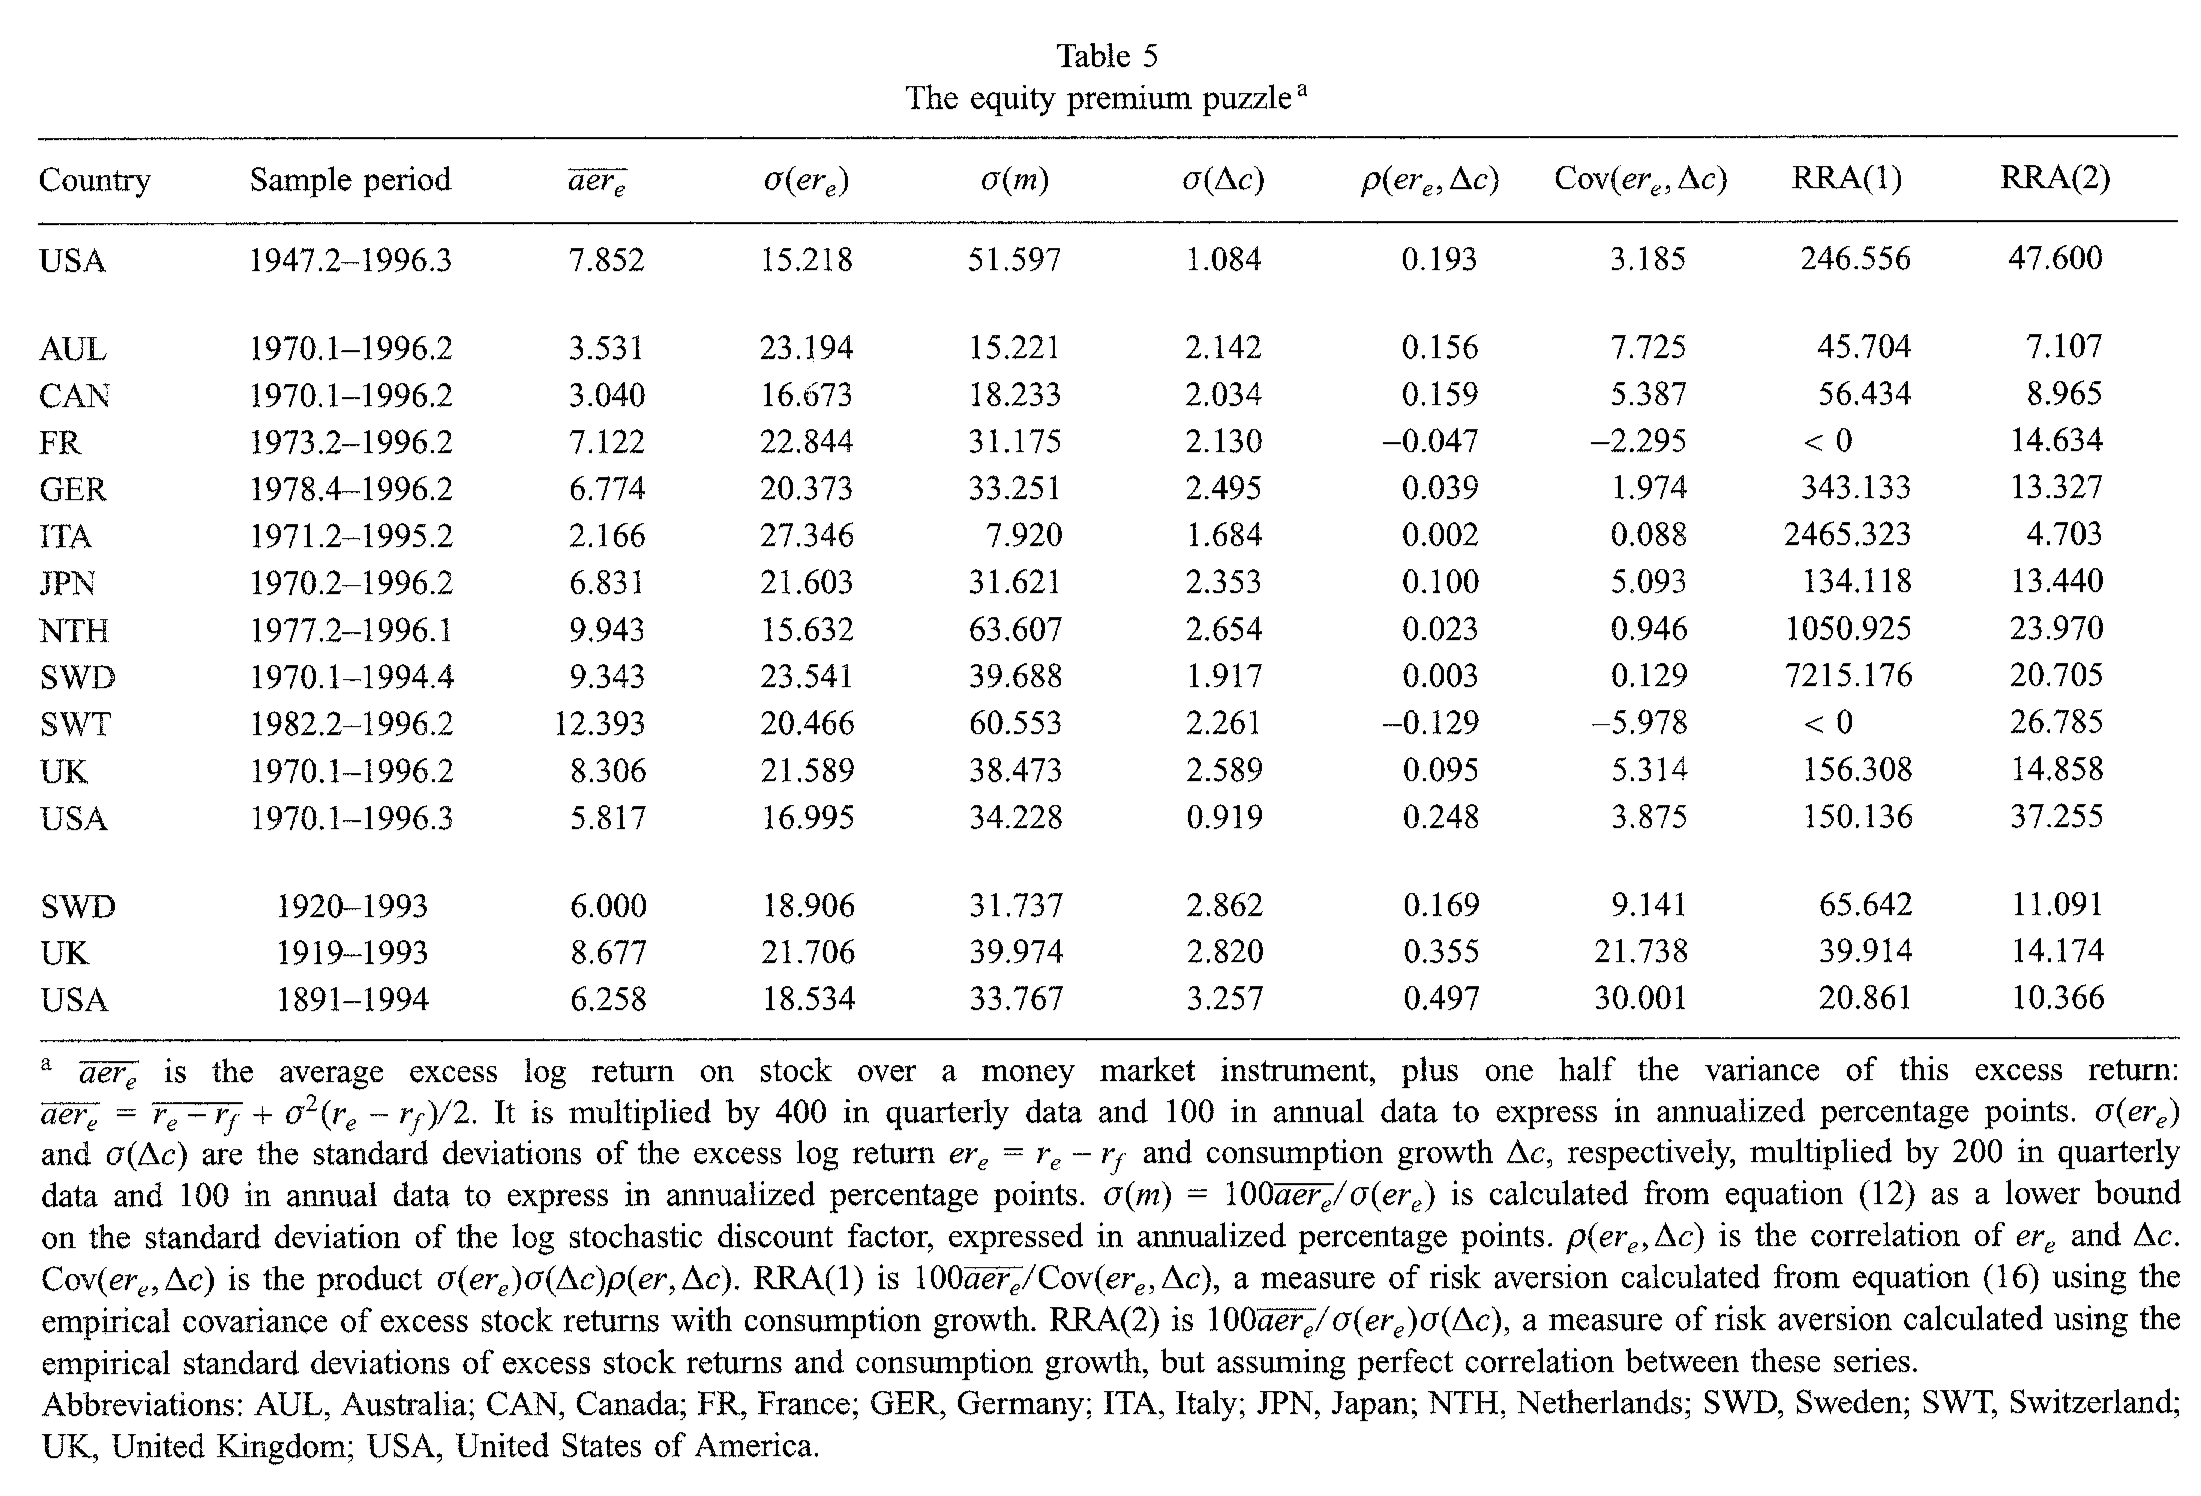
\includegraphics[width=.95\linewidth]{figures/table_campbell1999_eqpuzzle.pdf}
		\end{figure}
		\begin{tiny}
		\begin{center}
		Source: \href{http://www.sciencedirect.com/science/article/pii/S1574004899100326}{Campbell (1999)}.
		\end{center}
		\end{tiny}
\end{footnotesize}
\end{frame}

\begin{frame}\label{slide:rfpuzzle}
\begin{footnotesize}
\begin{itemize}
	\item For sake of comparison: microeconomic study points to estimates of $\gamma$ in $[1,3]$. \begin{scriptsize}[e.g. \href{http://www2.warwick.ac.uk/fac/soc/economics/research/workingpapers/2008/twerp719.pdf}{Hartley, Lanot and Walker, 2004}, \href{https://research.stlouisfed.org/wp/2014/2014-005.pdf}{Gandelman and Hernandez-Murillo (2014)}]\end{scriptsize}.
	\item[$\Rightarrow$] {\color{blue}Equity premium puzzle} put forward by \href{http://www.sciencedirect.com/science/article/pii/0304393285900613}{Mehra and Prescott (1985)}.
	\item \href{http://www.sciencedirect.com/science/article/pii/0304393291900048}{Kandel and Stambaugh (1991)}: Maybe that risk aversion is very high indeed?
	\item But then, another substantial problem arise: If people are very risk averse, they want to transfer consumption from high levels to low levels.
	\item In order to allow for a 2\% average increase in $C_t$, the model predicts that average short-term rate should be high (to prevent people from borrowing too much). Such high interest rates are at odds with the data.
	\item[$\Rightarrow$] {\color{blue}Risk-free rate puzzle}.
\end{itemize}
\end{footnotesize}
\end{frame}


\begin{frame}
\begin{footnotesize}
\begin{itemize}
	\item In the case of the power utility function, the risk aversion is the inverse of the Intertemporal Elasticity of Substitution (IES, Appendix \ref{def:IES}):
	$$
	\mbox{High risk aversion} \Leftrightarrow \mbox{Low IES [see Slide \ref{slide:gamma}]}.
	$$
	\item For given values of the risk-free rates $R_{f,t}$, a decrease in the IES (increase in $\gamma$) leads people to make consumption smoother [illustration on next slide].
	$$
	\frac{1}{1+R_{f,t}} \approx \mathbb{E}_t(\delta (1 - \gamma \Delta c_{t+1}))
	$$
	\item Hence, for the very large values of $\gamma$ necessary to fit average equity excess returns, agents strongly want to smoothen consumption.
	\item To reconcile a high risk aversion this with the observed low real interest rate observed on average, it must be that investors are infinitely patients ({\color{blue}risk-free rate puzzle}):
	If $\gamma=10$, $R_{f,t} \approx 0\%$ and $\Delta c_{t+1} \approx 2\%$, then $\delta \approx 1.25$, which is not reasonable.
\end{itemize}
\end{footnotesize}
\end{frame}


\begin{frame}
\begin{scriptsize}
\begin{exampleblock}{IES and smoothing behavior}
\begin{itemize}
	\item Two-period model. Power utility with $\delta=1$ and $R=5\%$.
	\item The agents have a wealth of 1 unit that they consume over two periods. If they consume $C_1$ in period, they consume $(1+R)(1-C_1)$ in period 2.
	\item The optimization of the intertemporal utility of the agents imply that $1/(1+R)=(C_2/C_1)^{-\gamma}$.
	\item[$\Rightarrow$] The lower the IES, the smoother the consumption path.
\end{itemize}
		\begin{figure}
			\includegraphics[width=.85\linewidth]{figures/Figure_PowerU_smoothing.pdf}
		\end{figure}
\end{exampleblock}
\end{scriptsize}
\end{frame}


\begin{frame}\label{slide:sharpepbm}
\begin{footnotesize}
\begin{itemize}
	\item A third problem pertains to the volatility of the s.d.f.
	
	[\href{https://www.jstor.org/stable/1815722?seq=1\#page_scan_tab_contents}{Grossman and Shiller (1981)}].
	\item \href{https://www.jstor.org/stable/2937680?seq=1\#page_scan_tab_contents}{Hansen and Jagannathan (1991)}: Sharpe ratios give lower bounds to the volatility of s.d.f.:
	$$
	\frac{\sigma_t(M_{t,t+1})}{\mathbb{E}_t(M_{t,t+1})} \ge \underbrace{\frac{\mathbb{E}_t(R_{i,t+1}-R_{f,t})}{\sigma_t(R_{i,t+1})}}_{\mbox{Sharpe ratio of asset $i$.}}
	$$
	(results from Eq. \ref{eq:MRCov}, using the fact that $\mathbb{C}ov(X,Y) \le \sigma(X)\sigma(Y)$)
	\item For postwar U.S. stock market, the Sharpe ratio is about 50\% [Slide \ref{slide:international}]. Given that $\mathbb{E}_t(M_{t,t+1}) \approx 1$, this imples that the volatility of the s.d.f. should be at least 50\%.
	\item For a power utility function [Def. \ref{def:RAmeasures}]:
	$$
	M_{t,t+1}=\delta (C_t/C_{t+1})^\gamma \approx (1 - \gamma \Delta c_{t+1}).
	$$
	Given the small volatility of $\Delta c_{t+1}$ [column $\sigma(\Delta c)$ in Slide \ref{slide:international}], $\gamma$ should be very high for the s.d.f. volatility to be equal to 50\%.
\end{itemize}
\end{footnotesize}
\end{frame}



\begin{frame}{Econometric Test of the C-CAPM: GMM}\label{slide:gmm}
\begin{footnotesize}
\begin{itemize}
	\item \href{https://www.jstor.org/stable/1911873?seq=1\#page_scan_tab_contents}{Hansen and Singleton (1982)} have developed and used the General Method of Moments to test the C-CAPM.
	\item This approach is based on the equation [Eq. \ref{eq:pricingcapm}]:
	\begin{equation}\label{eq:momentcondi}
	1 = {\color{red}\mathbb{E}_t}\left( \delta \left(\frac{C_t}{C_{t+1}}\right)^\gamma (1+R_{i,t+1})\right).
	\end{equation}
	\item For this to be verified, we must have, for any variable $z_t$:
	\begin{equation}\label{eq:GMM}
	{\color{red}\mathbb{E}}\left( \underbrace{\left[\delta \left(\frac{C_t}{C_{t+1}}\right)^\gamma (1+R_{i,t+1}) - 1\right] z_t}_{h_{t+1}}\right) = 0,
	\end{equation}
	\item[$\Rightarrow$] If not the case, one can use $z_t$ to predict $\delta \left(\frac{C_t}{C_{t+1}}\right)^\gamma (1+R_{i,t+1})$ and Eq. (\ref{eq:momentcondi}) is not valid. \hyperlink{slide:linearproj}{\beamergotobutton{Linear projections}}
	\item Moment condition: $\mathbb{E}(h_{t+1})=0$.

\end{itemize}
\end{footnotesize}
\end{frame}

\begin{frame}{Econometric Test of the C-CAPM: GMM}
\begin{footnotesize}
\begin{itemize}
	\item Empirical counterpart of the moment condition Eq. (\ref{eq:GMM}):
	\begin{equation}
	\frac{1}{T}\sum_{t=1}^{T} \left[\hat\delta \left(\frac{C_t}{C_{t+1}}\right)^{\hat\gamma} (1+R_{i,t+1}) - 1\right] \times\underbrace{z_{j,t}}_{\mbox{instrument}} = 0.
	\end{equation}
	\item In order to identify $\delta$ and $\gamma$, one need at least two such equations (with some $z_{1,t}$ and $z_{2,t}$).
	\item \href{https://www.jstor.org/stable/1911873?seq=1\#page_scan_tab_contents}{Hansen and Singleton (1982)} used lagged values of $R_{i,t+1}$ as instruments. \begin{tiny}[New York Stock Exchange indexes + indexes for different industries]\end{tiny}
	\item More than 2 equations = over-identification.
	\item One can use over-identifying restrictions to test for the model.
\end{itemize}
\end{footnotesize}
\end{frame}


\begin{frame}
\begin{scriptsize}
\begin{exampleblock}{\href{https://www.jstor.org/stable/1911873?seq=1\#page_scan_tab_contents}{Hansen and Singleton (1982)}}
\begin{itemize}
	\item Economically meaningful estimates with $\gamma$ ($=-\hat\alpha$ in the table below) close to unity (although with a large standard error) and $\delta$ ($=\hat\beta$ in the table below) slightly smaller than unity.
	\item However, when applied to more than one stock index, the over-identifying restrictions are generally rejected.
	\item[$\Rightarrow$] The data reject the simple version of CCAPM.
\end{itemize}
		\begin{figure}
			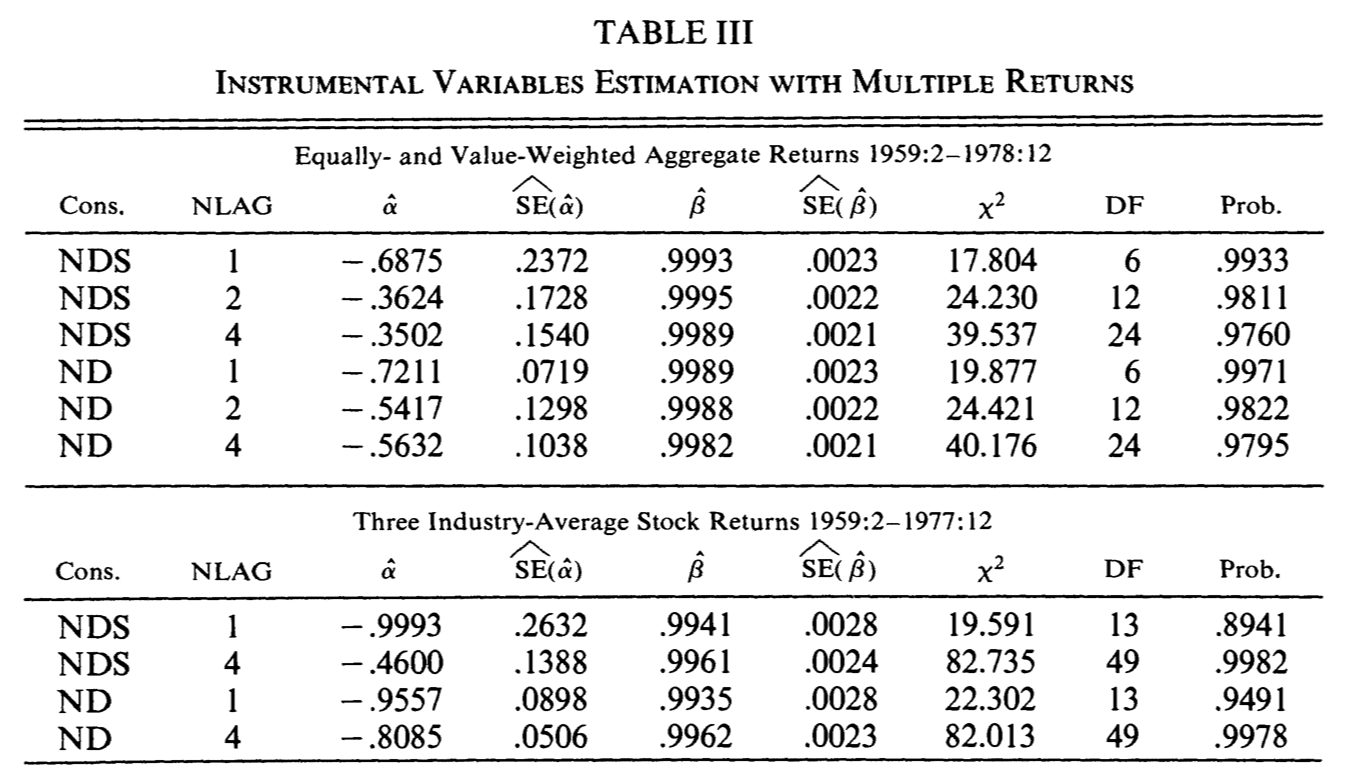
\includegraphics[width=.85\linewidth]{figures/tableHansenSingleton82A.pdf}
		\end{figure}
\end{exampleblock}
\end{scriptsize}
\end{frame}

\begin{frame}{C-CAPM: Playing with Data}
\begin{center}
Several of the previous results are illustrated

by this \href{https://jrenne.shinyapps.io/APModels}{web interface}.
\end{center}
\end{frame}



\begin{frame}{Long-run horizon}
\begin{scriptsize}
\begin{itemize}
	\item Stocks and consumption are more correlated at low frequencies [\href{https://jrenne.shinyapps.io/APModels}{web interface}].
	\item Hence equity-premium puzzle a little less strong for longer horizons [e.g. \href{http://journals.cambridge.org/action/displayAbstract?fromPage=online&aid=286196&fileId=S1365100597003076}{Daniel and Marshall, 1997}].
	\item \href{http://www.nber.org/papers/w11026}{Jagannathan and Wang (2005)}: CAPM not so bad when using fourth-quarter over fourth-quarter non-durable and service consumption [see next slide].
	
	\vspace{.2cm}
	Explanation?: A lot of purchases happen at Christmas, with an annual planning horizon (monthly horizon is maybe not relevant).
	
	\vspace{.2cm}
	Time aggregation = Spurious effect [Slide \ref{slide:spuriousXS}]? Maybe. But average excess returns line up  $\Rightarrow$ there is something here.
	
	\vspace{.2cm}
	\item \href{http://www.nber.org/papers/w9538}{Parker and Juillard (2005)}: study whether the 25 Fama-French portfolios can be priced when considering their exposure to "long-run" consumption risk. Formally, they study the condition:
	$$
	1 = \mathbb{E}_t \left( \beta \left(\frac{C_{t+k}}{C_t}\right)^{- \gamma} (1 + R_{i,t+1})(1 + R_{f,t+1})\times (1 + R_{f,t+k-1}) \right).
	$$
\end{itemize}
\end{scriptsize}
\end{frame}


\begin{frame}
\begin{footnotesize}
		\begin{figure}
			\includegraphics[width=.45\linewidth]{figures/chartJaganWang2005.pdf}
		\end{figure}
		\begin{tiny}
		\begin{center}
		Source:\href{http://www.nber.org/papers/w11026}{Jagannathan and Wang (2005)}.
		\end{center}
		\end{tiny}
\end{footnotesize}
\end{frame}



\begin{frame}{C-CAPM: That bad?}
\begin{footnotesize}
\begin{itemize}
	\item {\color{blue}Should we completely discard C-CAPM and the likes?}
	\item Constructive view of \href{http://faculty.chicagobooth.edu/john.cochrane/research/papers/financial_and_real_proofs_aug_07.pdf}{Cochrane (2007)}: The failure of the C-CAPM models is quantitative, not qualitative. In particular:
		\item[a.] Signs are consistent: since stock returns are positively correlated to consumption growth, the premiums have to be positive (which they are).
		\item[b.] The decrease in bond term premiums [Slide \ref{slide:ACMoench}] is consistent with decrease in the correlation between long-term bond excess returns and consumption [\href{https://jrenne.shinyapps.io/APModels}{web interface} and next slide].
		\item[c.] In terms of signs, the CAPM is also consistent with currency risk premiums [see Slide \ref{slide:currency}]:
		
		\href{http://web.mit.edu/adrienv/www/FX_Xsection.pdf}{Lustig and Verdelhan (2007)} show that high interest rate currencies depreciate on average when domestic consumption growth is low $\Rightarrow$ the CAPM predicts higher average return for investments in foreign high-interest rate currencies.
\end{itemize}
\end{footnotesize}
\end{frame}


\begin{frame}{Supply vs. Demand Shocks}
%\addtocounter{framenumber}{-1}
		\includegraphics[width=1.05\linewidth]{figures/Figure1b.pdf}
\end{frame}








